% !TEX root = ../root.tex

\chapter{Application: Geometric Control}

\begin{itemize_outcomes}
  \item Extend PD theory to Lie Groups.
  \item Model-predictive control
\end{itemize_outcomes}

\section{A Stabilizing Lie Group Controller}

Consider the system
\begin{equation}
  \begin{aligned}
    \mathrm{d}^r \X_t & = v \\
    \mathrm{d}^r v_t  & = u
  \end{aligned}
\end{equation}
where $u$ is a control input, and the objective of tracking a twice differentiable trajectory $\X_d(t)$ with first and second right-derivatives $v_d$ and $a_d$. Consider the error
\begin{equation}
  e_\X \coloneq \X_d \ominus_r \X,
\end{equation}
with derivative
\begin{equation}
  \mathrm{d}^r (e_\X)_t \overset{\eqref{eq:d_rminus_fst},\eqref{eq:d_rminus_snd}}= \left(\mathrm{d}^r \exp_{e_\X} \right)^{-1} \mathrm{d}^r \X_d - \left(\mathrm{d}^l \exp_{e_\X} \right)^{-1} \mathrm{d}^r \X = \left(\mathrm{d}^l \exp_{e_\X} \right)^{-1} (\bAd_{\exp(e_\X)} v_d - v).
\end{equation}
Note that $\bAd_{\exp(e_\X)} = \exp \ad_{e} = \sum_{k \geq 0} \frac{\ad_e}{k!}$ can typically be found on closed form via the usual expansion tricks. Let $e_v \coloneq \bAd_{\exp(e_\X)} v_d - v$ be the velocity error in the body frame; we then have the double intergrator-like error system
\begin{equation}
  \begin{aligned}
    \frac{\mathrm{d}}{\mathrm{d}t} e_\X & = \left(\mathrm{d}^l \exp_{e_\X} \right)^{-1} e_v,                        \\
    \frac{\mathrm{d}}{\mathrm{d}t} e_v  & = \frac{\mathrm{d}}{\mathrm{d}t} \left( \bAd_{\exp(e_\X)} v_d\right) - u,
  \end{aligned}
\end{equation}
Where we can further simplify
\begin{equation}
  \frac{\mathrm{d}}{\mathrm{d}t} \left( \bAd_{\exp(e_\X)} v_d\right) \overset{\eqref{eq:bAd_dl}}= \left[ \mathrm{d}^l \exp_{e_\X} \dot e_\X,  \bAd_{\exp(e_\X)} v_d \right] + \bAd_{\exp(e_\X)} \dot v_d = \left[ e_v,  \bAd_{\exp(e_\X)} v_d \right] + \bAd_{\exp(e_\X)} \dot v_d.
\end{equation}
If we further consider an input on the form $u = \left[ e_v,  \bAd_{\exp(e_\X)} v_d \right] + \bAd_{\exp(e_\X)} \dot v_d + k_p \textcolor{red}{\left( \mathrm{d}^l \exp_{e_\X} \right)^{-T}} e_\X + k_d e_v$ that cancels out the contribution from $v_d$ and adds PD feedback terms the closed-loop dynamics become
\begin{equation}
  \begin{aligned}
    \frac{\mathrm{d}}{\mathrm{d}t} e_\X & = \left(\mathrm{d}^l \exp_{e_\X} \right)^{-1} e_v,                                   \\
    \frac{\mathrm{d}}{\mathrm{d}t} e_v  & = -k_p \textcolor{red}{\left( \mathrm{d}^l \exp_{e_\X} \right)^{-T}} e_\X - k_d e_v.
  \end{aligned}
\end{equation}
Now consider a Lyapunov candidate function on the form
\begin{equation}
  V = \frac{k_p}{2} \| e_\X \|^2 + \frac{1}{2} \| e_v \|^2 + c \left \langle e_v, e_\X \right \rangle \geq \frac{1}{2} \begin{bmatrix} \| e_\X \| \\ \| e_v \| \end{bmatrix}^T \begin{bmatrix} k_p & -c \\ -c & 1 \end{bmatrix} \begin{bmatrix} \| e_\X \| \\ \| e_v \| \end{bmatrix},
\end{equation}
where $c$ is s.t. $k_p - c^2 \geq 0$ so that the matrix is positive definite. Its derivative evaluates to
\begin{equation*}
  \begin{aligned}
    \dot V & = k_p \left \langle e_\X, \left( \mathrm{d}^l \exp_{e_\X} \right)^{-1} e_v \right \rangle - k_p \left \langle e_v,  \textcolor{red}{\left( \mathrm{d}^l \exp_{e_\X} \right)^{-T}} e_\X \right \rangle - k_d \| e_v \|^2 + c \left \langle \dot e_v, e_\X \right \rangle + c \left \langle e_v, \dot e_\X \right \rangle \\
           & = - k_d \| e_v \|^2 - c \left \langle k_p \textcolor{red}{\left( \mathrm{d}^l \exp_{e_\X} \right)^{-T}} e_\X + k_d e_v, e_\X \right \rangle + c \left \langle e_v, \left(\mathrm{d}^l \exp_{e_\X} \right)^{-1} e_v \right \rangle                                                                                       \\
           & = -k_d \| e_v \|^2 - c k_p \| e_\X \|^2 - c k_d \left \langle e_v, e_\X \right \rangle + c \left \langle e_v, \left(\mathrm{d}^l \exp_{e_\X} \right)^{-1} e_v \right \rangle - c k_p \left \langle ( \textcolor{red}{(\mathrm{d}^l \exp_{e_\X})^{-T}} - I) e_\X , e_\X \right \rangle                                   \\
           & \leq -k_d \| e_v \|^2 - c k_p \| e_\X \|^2 + c k_d \| e_v \| \| e_\X \| + c \lambda_{\textrm{max}}\left( \left( \mathrm{d}^l \exp_{e_\X} \right)^{-1} \right) \| e_v \|^2 + c k_p \lambda_{\textrm{max}} \left( \textcolor{red}{\left(\mathrm{d}^l \exp_{e_\X} \right)^{-1}} - I \right) \| e_\X \|^2.
  \end{aligned}
\end{equation*}

\begin{itemize}
  \item Eigenvalues of $(\mathrm{d}^l \exp_{e_\X})^{-1}$ can be shown to be on the form $\frac{\lambda}{e^{\lambda} - 1} = \sum_{k=0}^\infty \frac{B_n}{n!} \lambda^n$, where $\lambda$ is an eigenvalue of $\ad_e$.
  \item Zero is always an eigenvalue of $\ad_e$ since $\ad_e e = 0$ due to it being a commutator (the corresponding eigenvalue of $(\mathrm{d}^l \exp_e)^{-1}$ is 1
  \item Often, eigenvalues of $\ad_e$ are purely imaginary. The corresponding eigenvalues of $(\mathrm{d}^l \exp_{e_\X})^{-1}$ are
        \begin{equation}
          \frac{i \lambda}{e^{i \lambda} - 1} = \frac{i \lambda e^{-i \lambda / 2}}{e^{i \lambda / 2} - e^{- i \lambda / 2}} = \frac{i \lambda e^{-i \lambda / 2}}{2 i \sin \lambda / 2} = \lambda \frac{\cos \lambda / 2 - i \sin \lambda / 2}{2 \sin \lambda / 2} = \frac{\lambda}{2} \cot \frac{\lambda}{2} - i \frac{\lambda}{2}.
        \end{equation}
        That is, the real part is equal to $\frac{\lambda}{2}\cot \frac{\lambda}{2}$.
  \item For angular groups we should throttle the angular part of $\| e_X \|$ at $\pm \pi/2$ in order to avoid the region where the eigenvalues approach zero which otherwise would lead to sluggish convergence
\end{itemize}

The maximal real part for $\lambda \in [-\pi, \pi]$ is attained at $\lambda = 0$ and is equal to 1, as shown in Figure \ref{fig:cot_fcn}. Thus, for lie groups s.t. $\ad_\a$ has purely imaginary eigenvalues in the range $[-\pi, \pi]$ for all $\a$, it holds that $\left( \mathrm{d}^l \exp_{e_\X} \right)^{-1}$ has no eigenvalue with real absolute magnitude larger than 1.

\begin{figure}
  \begin{center}
    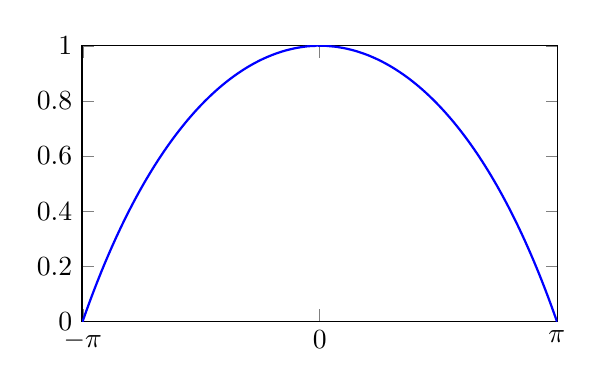
\begin{tikzpicture}
      \begin{axis}
        [
          width=3in,
          height=2in,
          xmin=-3.15,
          xmax=3.15,
          ymin=0,
          ymax=1,
          xtick={-3.14, 0, 3.1415},
          xticklabels={$-\pi$, 0, $\pi$},
        ]
        \addplot[no marks, thick, blue, samples=400]{x/2 * cot(deg(x/2))};
      \end{axis}
    \end{tikzpicture}
  \end{center}
  \caption{Function $x \mapsto \frac{x}{2} \cot \frac{x}{2}$.}
  \label{fig:cot_fcn}
\end{figure}

Let $\epsilon = \lambda_\textrm{max} \left( \textcolor{red}{\left(\mathrm{d}^l \exp_{e_\X} \right)^{-1}} - I \right)$; then we have
\begin{equation}
  \dot V \leq -\begin{bmatrix} \| e_\X \| \\ \| e_v \| \end{bmatrix}^T \begin{bmatrix} c k_p (1 - \epsilon) & -\frac{c k_d}{2} \\ -\frac{c k_d}{2} & k_d - c \end{bmatrix} \begin{bmatrix} \| e_\X \| \\ \| e_v \| \end{bmatrix}
\end{equation}
Therefore, if
\begin{equation}
  \begin{aligned}
    c k_p (1 - \epsilon) + k_d - c \geq 0 \\
    c k_p (1 - \epsilon) - \frac{c^2 k_d^2}{4}  \geq 0
  \end{aligned}
\end{equation}


In the following we let $M = SO(3)$ be the Lie group consisting of rotation matrices with matrix multiplication being the group action. We also write $e = I_3$ for the identity element of the group.

Consider the rigid body dynamics
\begin{subequations}
  \label{eq:attitude}
  \begin{align}
    \label{eq:attitude1} \dot R                 & = R \; {^R\hat \bomega},              \\
    \label{eq:attitude2} J \; {^R\dot{\bomega}} & = -{^R\hat\bomega} J {^R\bomega} + u,
  \end{align}
\end{subequations}
where $J$ is the moment of inertia, ${^R \hat \bomega} \in T M_R$ is the angular velocity in the body frame, and $R \in SO(3)$ is the attitude. We can see that the angular velocity ${^{e} \hat\bomega} \in T M_{e}$ in the inertial frame can be obtained as
\begin{equation}
  ^{e} \bomega = \Ad_R \left( ^R\bomega \right) = R {^R\bomega}.
\end{equation}
We also see that $^e \hat\bomega = \widehat {\Ad_R ^R\bomega } = R  \; {^R\bomega} \; R^T$, so it follows that \eqref{eq:attitude1} can be written as
\begin{equation}
  \dot R = {^e\hat\bomega} R.
\end{equation}

We assume that a smooth trajectory in the inertial frame is given by $R_d$ and $^e \bomega_d$ satisfying the dynamics
\begin{equation}
  \label{eq:desired_dyn}
  \dot R_d = {^e \hat \bomega_d} R_d,
\end{equation}
and the goal is to control $u$ in \eqref{eq:attitude} so that $R$ and $^e\bomega$ are close to $R_d$ and $^e\bomega_d$.

\section{Error Functions}

In general we would like to pick for $\tilde e_r = R_d \ominus R$ the error function $\frac{1}{2}\| \tilde e_r \|^2$ with derivative $\left\langle \tilde e_r, \tilde e_\bomega \right\rangle$ for
\begin{equation}
  \tilde e_\bomega = {\dot {\tilde e}}_r = {J^{R_d \ominus R}_{R_d}} \; {^{R_d} \bomega_d} + {J^{R_d \ominus R}_{R}} \; {^{R} \bomega}.
\end{equation}
This is general for any Lie group, and we can pick $u$ to stabilize a double integrator system in the tangent space. However, the derivative of $\tilde e_\bomega$ is cumbersome to evaluate and it is possible to arrive at a simpler formulation in $SO(3)$. Consider the error functions
\begin{subequations}
  \begin{align}
    \Psi(R, R_d) & = 1 - \cos(\theta) = \frac{1 - \tr(R R_d^T)}{2} = - \frac{1 - \left\langle R_d, R \right\rangle_F}{2}, \\
    e_r          & = \frac{1}{2} (R_d^T R-R^T R_d)^\vee,                                                                  \\
    e_\bomega    & = \bomega - R^T \bomega^d \in T SO(3)_R.
  \end{align}
\end{subequations}
It can be seen by \eqref{eq:so3_log} that $e_r$ is a rescaling of $\tilde e_r$. The derivative of $\Psi$ is $\left\langle e_r, e_\bomega \right\rangle$ as above, indeed
\begin{equation}
  \begin{aligned}
    \dot \Psi = & -\frac{1}{2} \left( \left\langle R_d, \dot R \right\rangle_F + \left\langle \dot R_d, R \right\rangle_F \right) = - \frac{1}{2} \left( \left\langle R_d , R \hat \bomega \right\rangle_F + \left\langle \hat \bomega_d R_d , R \right\rangle_F \right) =                             \\
                & = - \frac{1}{2} \left( \left\langle R^T R_d , \hat \bomega \right\rangle_F - \left\langle \hat \bomega_d^T R_d , R \right\rangle_F \right) = - \frac{1}{2} \left( \left\langle R^T R_d , \hat \bomega \right\rangle_F - \left\langle  R_d , \hat \bomega_d R \right\rangle_F \right) \\
                & = - \frac{1}{2} \left( \left\langle R^T R_d , \hat \bomega \right\rangle_F - \left\langle  R_d , R \widehat {R^T\bomega_d} \right\rangle_F \right) = - \frac{1}{2} \left\langle R^T R_d , \hat e_\bomega \right\rangle_F                         \\
                & = \frac{1}{4} \left\langle R_d^T R - R^T R_d, \hat e_\bomega \right\rangle_F = e_r \cdot e_\bomega,
  \end{aligned}
\end{equation}
where we have used the property that the Frobenius product $\left\langle A, B \right\rangle_F = - \left\langle A^T, B \right\rangle_F$ for $B$ skew-symmetric.

\todo[inline]{Do derivatives via jacobians instead}


\section{Lyapunov Stability}

We let the input be
\begin{equation}
  u = -k_r e_r - k_\bomega e_\bomega + \widehat{R^T \bomega_d} J R^T \bomega_d + J R^T \dot \bomega_d.
\end{equation}
and consider a Lyapunov candidate on the form
\begin{equation}
  V = \frac{1}{2} e_\bomega \cdot J e_\bomega + k_r \Psi + c e_r \cdot J e_\bomega
\end{equation}
The derivative of the Lyapunov candidate then \begin{proposition}
  It holds that
\end{proposition}
\begin{equation}
  \label{eq:myJeo_dot}
  J \dot e_\bomega = -k_r e_r - k_\bomega e_\bomega + \left( J e_\bomega + \left(2 J R^T \bomega_d - \text{trace}(J) I \right) R^T \bomega_d \right) \times e_\bomega.
\end{equation}
\begin{proof}
  \begin{equation*}
    \begin{aligned}
      \frac{\mathrm{d}}{\mathrm{d}t} J e_\bomega & \overset{\eqref{eq:e_omega}}= J \dot \bomega - J \dot R^T \bomega_d - J R^T \dot \bomega_d \overset{\eqref{eq:attitude}}= u - \hat \bomega J \bomega - J \left( R \hat \bomega \right)^T \bomega_d - J R^T \dot \bomega_d \\
                                                 & \overset{\eqref{eq:feedback}}= -k_r e_r - k_\bomega e_\bomega + \widehat{R^T \; {\bomega_d}} J R^T \; {\bomega_d} - \hat \bomega J \bomega - J \hat \bomega^T R^T \bomega_d                                               \\
                                                 & \overset{\eqref{eq:e_omega}}= -k_r e_r - k_\bomega e_\bomega + \widehat{R^T \; {\bomega_d}} J R^T \; {\bomega_d} - (\hat e_\bomega + \widehat{R^T \bomega_d}) J (e_\bomega + {R^T \bomega_d})   \\
                                                 & \quad + J \left( \hat e_\bomega + \cancelto{0}{\widehat{R^T \bomega_d}} \right) R^T \bomega_d                                                                                                                             \\
                                                 & = -k_r e_r - k_\bomega e_\bomega + \left( \widehat{J e_\bomega} + \widehat{J R^T \bomega_d} - \widehat{R^T \bomega_d} J - J \widehat{R^T \bomega_d} \right) e_\bomega                     \\
                                                 & = -k_r e_r - k_\bomega e_\bomega + \left( J e_\bomega + \left(2 J R^T \bomega_d - \text{trace}(J) I \right) R^T \bomega_d \right)^\wedge e_\bomega.
    \end{aligned}
  \end{equation*}
\end{proof}

We then get
\begin{equation}
  \begin{aligned}
    \dot V = -k_\bomega \| e_\bomega \|^2 + c \dot e_r \cdot J e_\bomega + c e_r \cdot J \dot e_\bomega
  \end{aligned}
\end{equation}
It remains to bound the terms involving $c$. We have that $\| \bomega \|_2^2 = \frac{1}{2} \| \hat \bomega \|_F^2$. We also have
\begin{equation}
  \frac{\mathrm{d}}{\mathrm{d}t} R_d^T R = R_d^T R \hat \bomega + R_d^T \hat \bomega_d^T R = R_d^T R \hat \bomega - R_d^T \hat \bomega_d R = R_d^T R \hat \bomega - R_d^T R \; \widehat{R^T \bomega_d} = R_d^T R \hat e_\bomega.
\end{equation}
and therefore we get that $\| \dot {\hat {e}}_r \|_F = \left\| \frac{1}{2} \left( R_d^T R \hat e_\bomega + \hat e_\bomega R^T R_d \right) \right\|_F \leq \| \hat e_\bomega \|_F$, so it follows that
\begin{equation}
  \| \dot e_r \|_2 \leq \| e_\bomega \|_2 \quad \implies \dot e_r \cdot J e_\bomega \leq \lambda_M(J) \| e_\bomega \|^2_2.
\end{equation}
Finally, using that $\| e_r \| \leq 1$,
\begin{equation}
  \begin{aligned}
    J \dot e_\bomega \cdot  e_r  \overset{\eqref{eq:myJeo_dot}}= \left( -k_r e_r - k_\bomega e_\bomega + \left( J e_\bomega + \left(2 J R^T \bomega_d - \text{trace}(J) I \right) R^T \bomega_d \right) \times e_\bomega \right) \cdot e_r \\
    \leq - k_r \| e_r \|^2 + k_\bomega \| e_r \| \| e_\bomega \| + \lambda_M(J) \| e_\bomega \|^2 + B \| e_\bomega \| \| e_r \|.
  \end{aligned}
\end{equation}
\begin{tcolorbox}
  We can now bound the derivative as follows:
  \begin{equation}
    \dot V \leq
    - \begin{bmatrix}
      \| e_r \| \\ \| e_\bomega \|
    \end{bmatrix}^T
    \begin{bmatrix}
      c k_r               & -c(k_\bomega + B)/2         \\
      -c(k_\bomega + B)/2 & k_\bomega - 2c \lambda_M(J)
    \end{bmatrix}
    \begin{bmatrix}
      \| e_r \| \\ \| e_\bomega \|
    \end{bmatrix},
  \end{equation}
  and it follows that if we choose $c$ small enough then the matrix is positive definite and thus $V$ decreases along trajectories of the closed-loop system.
\end{tcolorbox}


\section{Direction-driven Attitude Control on SO(3)}

We pick two orthogonal unit-length directions $b_1$ and $b_2$ and define the following error function:
\begin{equation}
  \Psi_i(R) = \frac{1}{2} \left\| R b_i - R_d b_i \right\|^2 = 1 - (R b_i) \cdot (R_d b_i).
\end{equation}
The derivative of $\Psi_i(R)$ becomes
\begin{equation}
  \label{eq:dot_psi}
  \begin{aligned}
    \dot \Psi_i(R) & = -\dot R b_i \cdot R_d b_i - R b_i \cdot \dot R_d b_i \overset{\eqref{eq:attitude1}, \eqref{eq:desired_dyn}}{=} -R {^R{\hat \bomega}} b_i \cdot R_d b_i - R b_i \cdot {^e\hat \bomega_d} R_d b_i                                                                                                                                   \\
                   & = - {^R{\hat \bomega}} b_i \cdot R^T R_d b_i - b_i \cdot R^T \; {^e\hat \bomega_d} R_d b_i = - {^R{\hat \bomega}} b_i \cdot R^T R_d b_i - b_i \cdot  \widehat{R^T \; {^e\bomega_d}} R^TR_d b_i                                                                                                \\
                   & = -{^R{\bomega}} \cdot \left( \widehat{b_i} \; R^T R_d b_i \right) - R^T \; {^e\bomega_d} \cdot \widehat{R^TR_d b_i} b_i = \underbrace{\left( {^R{ \bomega}} - R^T \; {^e\bomega_d} \right)}_{e_\bomega} \cdot \underbrace{\widehat{R^TR_d b_i} b_i}_{e_{r_i}},
  \end{aligned}
\end{equation}
where we have defined two error functions
\begin{subequations}
  \begin{align}
    \label{eq:e_ri} e_{r_i}      & = \widehat{R^TR_d b_i} b_i,           \\
    \label{eq:e_omega} e_\bomega & = {^R\bomega} - R^T \; {^e\bomega_d},
  \end{align}
\end{subequations}
that are small when $R \approx R_d$ and when $\Ad_R {^R{\hat \bomega}} = R {^R{\hat \bomega}} \approx {^e\bomega_d}$, respectively.

\section{Feedback Control}

\begin{tcolorbox}
  Given these error functions we consider the feedback control
  \begin{equation}
    \label{eq:feedback}
    u = -e_r - k_\bomega e_\bomega + \widehat{R^T \; {^e\bomega_d}} J R^T \; {^e\bomega_d} + J R^T {^e\dot \bomega_d},
  \end{equation}
  where
  \begin{equation}
    \label{eq:er}
    e_r = k_1 e_{r_1} + k_2 e_{r_2},
  \end{equation}
  and $k_1, k_2, k_\bomega$ are positive gains. Take the candidate Lyapunov function
  \begin{equation}
    V = \frac{1}{2} e_\bomega \cdot J e_\bomega + k_1 \Psi_1(R) + k_2 \Psi_2(R) + c J e_\bomega \cdot e_r.
  \end{equation}
\end{tcolorbox}

In the following we drop the upper left superscripts and write $\bomega = {^R\bomega}$ and $\bomega_d = {^e\bomega_d}$.


\section{Lyapunov lower bound}
We would like to show that $V = 0$ implies that $\| e_r \|$ and $\| e_\bomega \|$ are zero. The main challenge lies in bounding the terms containing $\Psi_i$. Note that
\begin{equation}
  \label{eq:eri_sin}
  \|e_{r_i}\| = \|\widehat{R^TR_d b_i} b_i\| = \|R^TR_d b_i \times b_i\| = \sin \theta_i,
\end{equation}
where $\theta_i$ is the angle between $R^TR_d b_i$ and $b_i$. Note that $\theta_i$ is always in the range $[0, \pi]$. Similarly,
\begin{equation}
  \label{eq:psi_cos}
  \Psi_i(R) = 1 - R^T R_d b_i \cdot b_i = 1 - \cos \theta_i.
\end{equation}
Utilizing this and $(a+b)^2 \leq 2(a^2 + b^2)$ we get:
\begin{equation*}
  \begin{aligned}
    \| e_r \|^2 & \overset{\eqref{eq:er}}= \| k_1 e_{r_1} + k_2 e_{r_2} \|^2 \leq ( k_1 \| e_{r_1} \| + k_2 \| e_{r_2} \| )^2 \overset{\eqref{eq:eri_sin}}= ( k_1 \sin \theta_1 + k_2 \sin \theta_2 )^2 \\
                & = \left( k_1 \sqrt{1 - \cos^2 \theta_1 } + k_2 \sqrt{1 - \cos^2 \theta_2 } \right)^2 \leq \left( k_1 \sqrt{2(1 - \cos \theta_1)} + k_2 \sqrt{2(1 - \cos \theta_2) } \right)^2         \\
                & \overset{\eqref{eq:psi_cos}}= 2 \left( k_1 \sqrt{\Psi_1(R)} + k_2 \sqrt{\Psi_2(R)} \right)^2 \leq 4 \min(k_1, k_2) \left( k_1\Psi_1(R) + k_2\Psi_2(R) \right).
  \end{aligned}
\end{equation*}
\begin{tcolorbox}
  We therefore get
  \begin{equation}
    V \geq \frac{1}{2} \begin{bmatrix}
      \| e_r \| \\ \| e_\bomega \|
    \end{bmatrix}^T
    \begin{bmatrix}
      \frac{1}{2\min(k_1, k_2)} & -c \lambda_M(J) \\
      -c \lambda_M(J)           & \lambda_m(J)
    \end{bmatrix}
    \begin{bmatrix}
      \| e_r \| \\ \| e_\bomega \|
    \end{bmatrix}
  \end{equation}
  where the matrix is positive definite for small enough $c$.
\end{tcolorbox}

\section{Lyapunov derivative}

We start with an intermediate result
\begin{proposition}
  It holds that
\end{proposition}
\begin{equation}
  \label{eq:Jeo_dot}
  J \dot e_\bomega = -e_r - k_\bomega e_\bomega + \left( J e_\bomega + \left(2 J R^T \bomega_d - \text{trace}(J) I \right) R^T \bomega_d \right) \times e_\bomega.
\end{equation}
\begin{proof}
  \begin{equation*}
    \begin{aligned}
      \frac{\mathrm{d}}{\mathrm{d}t} J e_\bomega & \overset{\eqref{eq:e_omega}}= J \dot \bomega - J \dot R^T \bomega_d - J R^T \dot \bomega_d \overset{\eqref{eq:attitude}}= u - \hat \bomega J \bomega - J \left( R \hat \bomega \right)^T \bomega_d - J R^T \dot \bomega_d \\
                                                 & \overset{\eqref{eq:feedback}}= -e_r - k_\bomega e_\bomega + \widehat{R^T \; {\bomega_d}} J R^T \; {\bomega_d} - \hat \bomega J \bomega - J \hat \bomega^T R^T \bomega_d                                                   \\
                                                 & \overset{\eqref{eq:e_omega}}= -e_r - k_\bomega e_\bomega + \widehat{R^T \; {\bomega_d}} J R^T \; {\bomega_d} - (\hat e_\bomega + \widehat{R^T \bomega_d}) J (e_\bomega + {R^T \bomega_d})       \\
                                                 & \quad + J \left( \hat e_\bomega + \cancelto{0}{\widehat{R^T \bomega_d}} \right) R^T \bomega_d                                                                                                                             \\
                                                 & = -e_r - k_\bomega e_\bomega + \left( \widehat{J e_\bomega} + \widehat{J R^T \bomega_d} - \widehat{R^T \bomega_d} J - J \widehat{R^T \bomega_d} \right) e_\bomega                         \\
                                                 & = -e_r - k_\bomega e_\bomega + \left( J e_\bomega + \left(2 J R^T \bomega_d - \text{trace}(J) I \right) R^T \bomega_d \right)^\wedge e_\bomega.
    \end{aligned}
  \end{equation*}
\end{proof}
Thus the derivative of $V$ is
\begin{equation}
  \begin{aligned}
    \dot V \overset{\eqref{eq:dot_psi}}= e_\bomega \cdot J \dot e_\bomega + e_r \cdot e_\bomega + c J \dot e_\bomega \cdot e_r + c J e_\bomega \cdot \dot e_r
    \overset{\eqref{eq:Jeo_dot}}= -k_\bomega \| e_\bomega \|^2 + c J \dot e_\bomega \cdot e_r + c J e_\bomega \cdot \dot e_r,
  \end{aligned}
\end{equation}
so we would like to bound $J \dot e_\bomega \cdot e_r$ and $J e_\bomega \cdot \dot e_r$ in terms of $\| e_\bomega \|$ and $\| e_r \|$.  First we have
\begin{equation}
  \label{eq:rdr_dt}
  \frac{\mathrm{d}}{\mathrm{d}t} R_d^T R = R_d^T R \hat \bomega + R_d^T \hat \bomega_d^T R  = R_d^T R \hat \bomega - R_d^T \hat \bomega_d R = R_d^T R \hat \bomega - R_d^T R \; \widehat{R^T \bomega_d} = R_d^T R \hat e_\bomega.
\end{equation}
Now, $e_{r_i} = \widehat{R^T R_d b_i} b_i,$ so by linearity of the hat mapping and that $\| \hat b_i \| = \| b_i \| = 1$ it follows that
\begin{equation}
  \dot e_{r_i} = \widehat{R_d^T R \hat e_\bomega b_i} \; b_i = - \widehat{R_d^T R \hat b_i e_\bomega} \; b_i, \quad \implies \| \dot e_{r_i} \| \leq \| R_d^T R \| \| \hat b_i \| \| e_\bomega \| \| b_i \| = \| e_\bomega \|.
\end{equation}
Thus, for $\lambda_M(J)$ the maximal eigenvalue of $J$,
\begin{equation}
  \| J e_\bomega \cdot \dot e_r \| \leq \lambda_M(J) (k_1 + k_2) \| e_\bomega \|^2.
\end{equation}
Finally, we bound the last term, utilizing that $\| e_r \| \leq k_1 + k_2$:
\begin{equation}
  \begin{aligned}
    J \dot e_\bomega \cdot  e_r  \overset{\eqref{eq:Jeo_dot}}= \left( -e_r - k_\bomega e_\bomega + \left( J e_\bomega + \left(2 J R^T \bomega_d - \text{trace}(J) I \right) R^T \bomega_d \right) \times e_\bomega \right) \cdot e_r \\
    \leq - \| e_r \|^2 + k_\bomega \| e_r \| \| e_\bomega \| + \lambda_M(J) (k_1 + k_2) \| e_\bomega \|^2 + B \| e_\bomega \| \| e_r \|,
  \end{aligned}
\end{equation}
where $B$ is some number that upper bounds $\| \left( 2 J R^T \bomega_d - \text{trace}(J) I \right) R^T \bomega_d \|$.

\begin{tcolorbox}
  We can now bound the derivative as follows:
  \begin{equation}
    \dot V \leq
    - \begin{bmatrix}
      \| e_r \| \\ \| e_\bomega \|
    \end{bmatrix}^T
    \begin{bmatrix}
      c                   & -c(k_\bomega + B)/2                     \\
      -c(k_\bomega + B)/2 & k_\bomega - 2c \lambda_M(J) (k_1 + k_2)
    \end{bmatrix}
    \begin{bmatrix}
      \| e_r \| \\ \| e_\bomega \|
    \end{bmatrix},
  \end{equation}
  and it follows that if we choose $c$ small enough then the matrix is positive definite and thus $V$ decreases along trajectories of the closed-loop system.
\end{tcolorbox}

\textbf{Remaining steps:}

\begin{itemize}
  \item Show that undesired equilibria are unstable
\end{itemize}


\chapter{Application: Model-Predictive Control}

Consider a system $\X(t)$ evolving on a Matrix Lie group
\begin{equation}
  \label{eq:mpc_dynamics}
  \mathrm{d}^r \X_t = f(\X, u), \quad \X \in \M, \qquad f : \M \times U \rightarrow T \M.
\end{equation}
We are interested in finding an approximate solution to the optimal control problem
\begin{equation}
  \label{eq:mpc_ocp}
  \begin{cases}
    \min        & \int_0^T \left\| \sqrt{Q(\tau)} (\X(\tau) \ominus_r \X_d(\tau)) \right\|_2^2 + \left\| \sqrt{R(\tau)} (u(\tau) - u_d(\tau)) \right\| \mathrm{d} \tau + \left\| \sqrt{Q(T)} (\X(T) \ominus_r x_d(T)) \right\|_2^2 \\
    \text{s.t.} & \eqref{eq:mpc_dynamics}                                                                                                                                                                                          \\
                & \X(0) = \X_0
  \end{cases},
\end{equation}
for positive semi-definite matrices $Q$ and $R$.

We start by considering the dynamics around a nominal trajectory $(\X_l(t), u_l(t))$. Consider the error $\a_e = \X(t) \ominus_r \X_l(t)$. Since the error takes values in $T_{\X_l(t)} \M \cong \mathbb{R}^n$ the rule of total derivatives in Remark \ref{remark:total_derivative} applies and the error dynamics become
\begin{equation}
  \label{eq:mpc_linearized_dynamics}
  \begin{aligned}
    \frac{\mathrm{d} \a_e}{\mathrm{d}t} = \mathrm{d}^r (\a_e)_t
     & = \mathrm{d}^r (\X \ominus_r \X_l)_\X \mathrm{d}^r \X_t + \mathrm{d}^r (\X \ominus_r \X_l)_{\X_l} \; \mathrm{d}^r (\X_l)_t
    \\
     & \overset{\eqref{eq:d_rminus_fst}, \eqref{eq:d_rminus_snd}}= \left[\mathrm{d}^r \exp_{\a_e} \right]^{-1} f\left(\X_l \oplus_r \a_e, u_l + u_e \right) - \left[\mathrm{d}^l \exp _{\a_e} \right]^{-1} \; \mathrm{d}^r (\X_l)_t,
  \end{aligned}
\end{equation}
Thus we can change coordinates and rewrite \eqref{eq:mpc_ocp} as
\begin{equation}
  \label{eq:mpc_ocp_error}
  \begin{cases}
    \min        & \int_0^T \left\| \sqrt{Q(\tau)} \left( \left( \X_l(\tau) \oplus_r \a_e(\tau) \right) \ominus_r \X_d(\tau) \right)  \right\|_2^2 + \left\| \sqrt{R(\tau)} (u_l(\tau) + u_e(\tau) - u_d(\tau)) \right\|  \mathrm{d} \tau, \\

    \text{s.t.} & \eqref{eq:mpc_linearized_dynamics},                                                                                                                                                                                     \\
                & \a_e(0) = \X_0 \ominus \X_l(0).
  \end{cases},
\end{equation}
This is now a regular optimal control problem and we can proceed by linearizing around $(\a_e, u_e) = (0, 0)$ to obtain the linear time-varying system:
\begin{equation}
  \frac{\mathrm{d}}{\mathrm{d}t} \a_e = A(t) \a_e + B(t) u_e + E(t),
\end{equation}
where, since $\mathrm{d}^r \exp_0 = \mathrm{d}^l \exp_0 = I$,
\begin{align}
  A(t) & \coloneq \left. \frac{\mathrm{d}}{\mathrm{d}\a_e} \right|_{\a_e = 0} \left[\mathrm{d}^r \exp_{\a_e} \right]^{-1} f\left(\X_l(t) \oplus_r \a_e, u_l(t)  \right),  \\
  B(t) & \coloneq \left. \frac{\mathrm{d}}{\mathrm{d}u_e} \right|_{u_e = 0} f\left(\X_l(t), u_l(t) + u_e \right),  \\
  E(t) & \coloneq f\left(\X_l(t), u_l(t) \right) - \mathrm{d}^r(\X_l)_t.
\end{align}
To facilitate evaluating the cost function we note that
\begin{equation}
  \left( \X_l \oplus_r \a_e \right) \ominus_r \X_d = \log \left( \X_d^{-1} \circ \X_l \circ \exp(\a_e) \right) = \log(\exp(\X_l \ominus_r \X_d) \circ \exp(\a_e)) \approx \X_l \ominus_r \X_d + \a_e(t),
\end{equation}
where the last approximate step follows from the Baker-Campbell-Hausdorff formula \eqref{eq:bch_formula}.

We can thus write it on the form
\begin{equation}
  \left\| \sqrt{Q} \left( \left( \X_l \oplus_r \a_e \right) \ominus_r \X_d \right)  \right\|_2^2 \approx \left( \X_l \ominus_r \X_d + \a_e \right)^T Q \left( \X_l \ominus_r \X_d + \a_e \right) = \a_e^T Q \a_e + 2\left( \X_l \ominus_r \X_d  \right)^T Q \a_e.
\end{equation}
